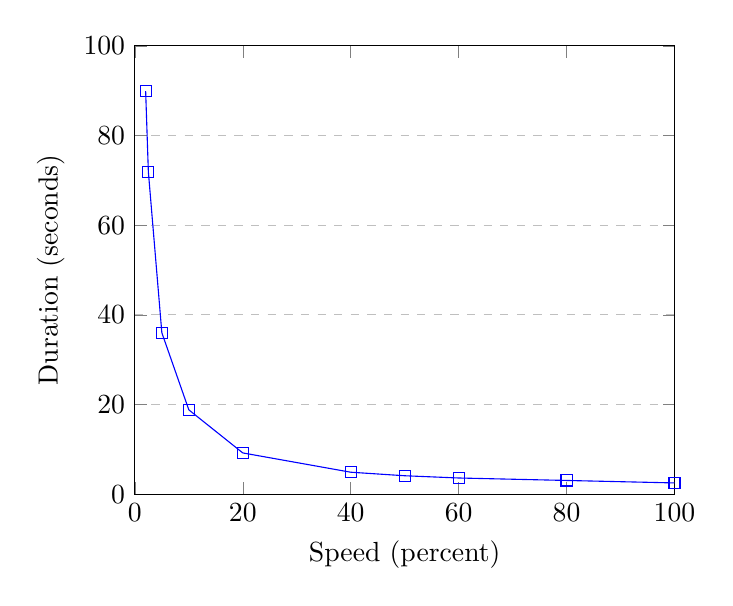
\begin{tikzpicture}
\begin{axis}[
%    title={Relation of operation duration to robot speed},
    xlabel={Speed (percent)},
    ylabel={Duration (seconds)},
    xmin=0, xmax=100,
    ymin=0, ymax=100,
    xtick={0,20,40,60,80,100},
    ytick={0,20,40,60,80,100},
    legend pos=north west,
    ymajorgrids=true,
    grid style=dashed,
]
 
\addplot[
    color=blue,
    mark=square,
    ]
    coordinates {
    (100, 2.5)(80, 3.05)(60, 3.6)(50, 4.1)(40, 4.89)(20, 9.19)(10, 18.8)(5, 36)(2.5, 71.93)(2, 89.9)
    };
\end{axis}
\end{tikzpicture}